%//==============================--@--==============================//%
\subsection[3.1 Transístor de junção bipolar (BJT)]{\hspace*{0.075 em}\raisebox{0.2 em}{$\pmb{\drsh}$} Transístor de junção bipolar (BJT)}
\label{subsec:transístor-BJT}

O \textbf{transístor de junção bipolar} ou \textbf{transístor bipolar} (BJT) pode ser visto como um dispositivo de três terminais, descrito em termos das suas correntes e tensões; a designação de "bipolar" resulta da intervenção de cargas negativas (eletrões) e positivas (lacunas) no seu funcionamento (em contraste com os MOSFET que veremos mais adiante).

\begin{figure}[H]
    \centering
    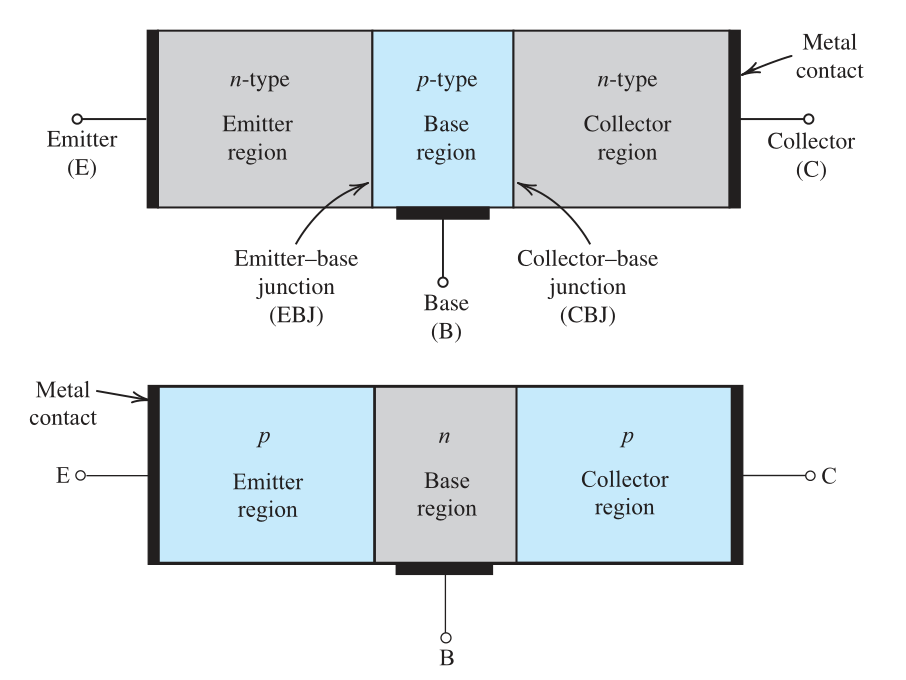
\includegraphics[width=0.7\linewidth]{img/3/BJT/npn-pnp-structure.png}
    \caption{``A simplified structure of the \textit{npn}/\textit{pnp} transistor.''\cite{sedra-smith:microelectronic-circuits}}
    \label{fig:npn-pnp-structure}
\end{figure}

\begin{itemize}[leftmargin=*]
    \item \textbf{Estrutura simplificada do BJT:} Um transístor bipolar consiste em três regiões de semicondutores: o \textbf{emissor}, a \textbf{base} e o \textbf{coletor}. Os terminais são conectados a cada região e identificados como E (emissor), B (base) e C (coletor). 
    
    Existem dois tipos de BJTs: \textbf{npn} (emissor tipo n, base tipo p e coletor tipo n) e \textbf{pnp} (emissor tipo p, base tipo n e coletor tipo p).
    
    \item O BJT admite duas junções pn, a \textbf{junção emissor-base} (EBJ) e a \textbf{junção coletor-base} (CBJ).
    
    \item \textbf{Modos de operação:} Consoante a polarização das regiões EBJ e CBJ, obtêm-se diferentes modos de operação:
    {
    \setlength{\tabcolsep}{14pt}
    
    \begin{table}[h!]
        \centering
        \captionsetup{justification=centering}
        \caption{``BJT Modes of Operation''\cite{sedra-smith:microelectronic-circuits} (para npn)}
        \label{tab:}
        \begin{tabularx}{0.55\textwidth}{lll}
            \toprule
            \multicolumn{1}{c}{\textbf{Mode}} & \multicolumn{1}{c}{\textbf{EBJ}} & \multicolumn{1}{c}{\textbf{CBJ}} \\
            \midrule
            Cutoff & Reverse & Reverse \\
            Saturation & Forward & Forward \\
            Active & Forward & Reverse \\
            \color{gray} Reverse Active & \color{gray} Reverse & \color{gray} Forward \\
            \bottomrule
        \end{tabularx}
    \end{table}
    }
    O \textit{\underline{modo de corte}} e o \textit{\underline{modo de saturação}} são usualmente utilizados em aplicações digitais (aplicações de interruptor $[$on/off$]$, circuitos lógicos, ...); enquanto o \textit{\underline{modo ativo}} serve maioritariamente para amplificação (comummente para uso analógico).
\end{itemize}

%//==============================--@--==============================//%
\subsubsection[3.1.1 Modos de operação]{$\pmb{\rightarrow}$ Modos de operação}

\begin{figure}[H]
    \centering
    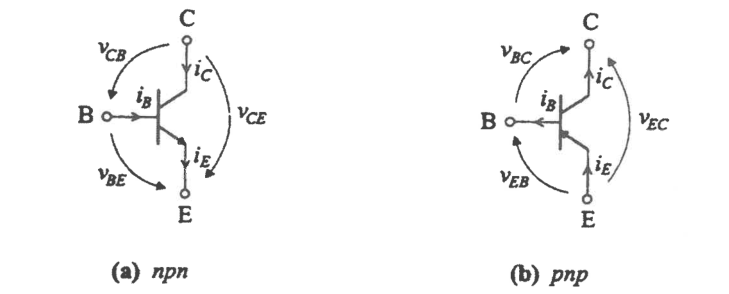
\includegraphics[width=0.7\linewidth]{img/3/BJT/BJT-symbol.png}
    \caption{``Símbolo dos transístores bipolares e sentidos de referência.''\cite{medeiros:CTBM}}
    \label{fig:BJT-symbol}
\end{figure}

\begin{quote}
    ``O funcionamento dos dois tipos de transístores é muito semelhante: quando se passa de um para o outro, todos os resultados se mantêm se se trocarem os sentidos das correntes e tensões.''\cite{medeiros:CTBM} 
\end{quote}

\noindent Na subsequente análise é \underline{considerado o transístor npn} dado que é o mais frequentemente utilizado.

\vspace{0.5em}
\noindent Das leis de Kirchhoff resulta que
$$
    \text{KCL}\; \boxed{ i_E = i_C + i_B } \mkern38mu \text{KVL}\; \boxed{ v_{CB} = v_{CE} - v_{BE} }
$$
$\implies$ para caracterizar o estado do transístor, basta indicar duas correntes e duas tensões.

%//==============================--@--==============================//%
\paragraph[3.1.1.1 Modo Ativo (ZAD)]{$\pmb{\star}$ Modo Ativo (ZAD)}\mbox{}

\begin{figure}[H]
    \centering
    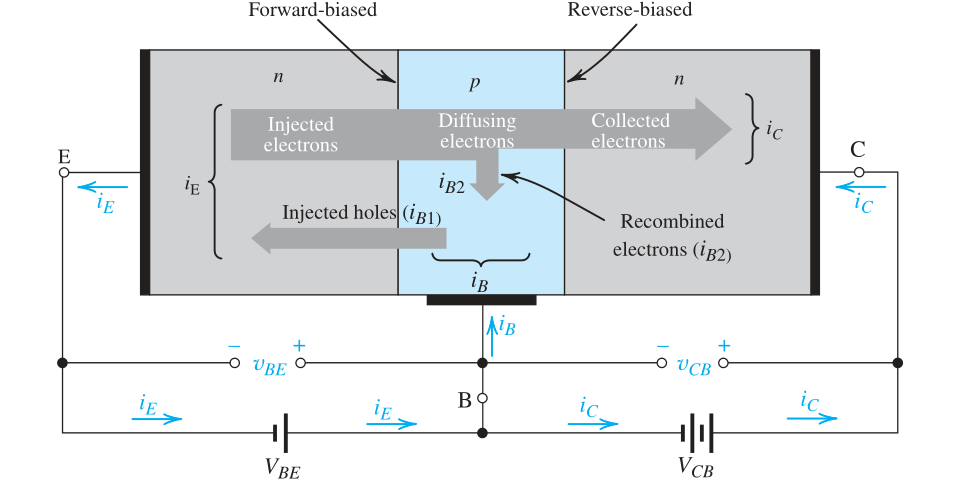
\includegraphics[width=0.75\linewidth]{img/3/BJT/active-mode.png}
    \caption{``Current flow in an npn transistor biased to operate in the active mode. (Reverse current
components due to drift of thermally generated minority carriers are not shown.)''\cite{sedra-smith:microelectronic-circuits}}
    \label{fig:active-mode}
\end{figure}

\noindent De modo a ilustrar o modo de operação do transístor no modo ativo, apresentam-se na \hyperref[fig:active-mode]{Fig. 21} duas fontes de tensão externas, $V_\textit{BE}$ e $V_\textit{CB}$, que verificam $v_\textit{CB} \ge v_\textit{BE}$.

\begin{itemize}[leftmargin=*]
    \item A tensão $V_\textit{BE}$ coloca a base de tipo p a um potencial superior ao emissor de tipo n, estabelecendo uma polarização direta na junção emissor-base (\textit{forward bias}). 
    
    \item A tensão coletor-base $V_\textit{CB}$, força o coletor de tipo n a um maior potencial relativamente à base, o que resulta numa polarização inversa para a junção coletor-base (\textit{reverse bias}).
\end{itemize}

\begin{itemize}[leftmargin=*]
    \item[] \textbf{Fluxo de corrente}:
    \begin{itemize}[leftmargin=*,label=$\pmb{-}$]
        \item A polarização direta da EBJ provoca o fluxo de corrente, composto por dois componentes: eletrões injetados do emissor para a base, e lacunas injetadas (de- sejavelmente, em menor quantidade) da base para o emissor.
        \item A magnitude da corrente do emissor, $i_E$, é dominada pelo componente maioritário (eletrões no caso do transístor npn).
        \begin{quote}
            ``The direction of $i_E$ is "out of" the emitter lead, which, following the usual conventions, is in the direction of the positive-charge flow (hole current) and opposite to the direction of the negative-charge flow (electron current), with the emitter current $i_E$ being equal to the sum of these two components. However, since the electron component is much larger than the hole component, the emitter current will be dominated by the electron component.''\cite{sedra-smith:microelectronic-circuits}
        \end{quote}
        \item As correntes do emissor e da base são proporcionais a $e^{v_\textit{BE}/V_T}$, onde $v_\textit{BE}$ é a tensão direta da junção base-emissor e $V_T \simeq 25$ mV é a tensão térmica (junção pn).
    \end{itemize}
    
    \item[] \textbf{Corrente do coletor}:
    \begin{itemize}[leftmargin=*,label=$\pmb{-}$]
        \item A maioria dos eletrões injetados do emissor para a base chega ao coletor, criando a corrente do coletor ($i_C$):
        $$
            i_C = I_S \left(e^{\frac{v_\textit{BE}}{V_T}} - 1\right) \simeq I_S\, e^{\frac{v_\textit{BE}}{V_T}},\quad \text{onde $I_S$ é a corrente de saturação}
        $$
    \end{itemize}
    
    \item[] \textbf{Corrente da base}:
    \begin{itemize}[leftmargin=*,label=$\pmb{-}$]
        \item A corrente da base ($i_B$) é composta por duas componentes: lacunas injetadas da base para o emissor e lacunas necessárias para o processo de \textbf{recombinação}\footnotemark[4] na base (também proporcionais a $e^{v_\textit{BE}/V_T}$). A corrente na base pode ser expressa como:
        $$
            i_B = \frac{i_C}{\beta},\quad \text{onde $\beta$ é o \textbf{ganho de corrente de emissor comum}}
        $$
    \end{itemize}
    
    \item[] \textbf{Corrente do emissor}:
    \begin{itemize}[leftmargin=*,label=$\pmb{-}$]
        \item A corrente do emissor ($i_E$) é a soma da corrente do coletor e da corrente da base.
        $$ i_E = i_C + i_B = \frac{\beta + 1}{\beta}\, i_C $$
        Alternativamente, é possível exprimir a fórmula na seguinte forma:
        $$ i_C = \alpha\, i_E $$
        em que a contante $\alpha$ se relaciona com $\beta$ por
        $$ \alpha = \frac{\beta}{\beta + 1} \iff \beta = \frac{\alpha}{1-\alpha}$$ 
        Como veremos mais adiante, $\alpha$ é também denominado por \textbf{ganho de corrente de base comum}.
    \end{itemize}
\end{itemize}

\footnotetext[4]{%
    Os eletrões injetados do emissor para a base são portadores minoritários na região da base tipo p. Durante a jornada até ao coletor, alguns eletrões combinam-se com lacunas (portadores de carga maioritários) na base. No entanto, como a base é geralmente muito fina e pouco dopada, a proporção de eletrões perdidos neste processo de recombinação é bastante pequena. A maioria dos eletrões difundidos alcança a fronteira da região de depleção coletor-base e, devido à tensão de polarização inversa ($v_\textit{CB}$) aplicada entre o coletor e a base, são varridos através da região de depleção, chegando finalmente ao coletor e constituindo a corrente do coletor $i_C$.
}

%//==============================--@--==============================//%
\paragraph[3.1.1.2 Modo de Saturação (\textit{Saturation})]{$\pmb{\star}$ Modo de Saturação (\textit{Saturation}\footnotemark[5])}\mbox{}

\vspace{-0.40em}
\begin{center}
    \begin{minipage}{0.65\linewidth}
        $v_{BE} = v_{CE} \simeq 0.7$V, de forma a que $i_C > 0$ e $i_B > 0$, mas $i_C < \beta i_B$. O transístor está plenamente saturado quando $v_{CE} = V_{CE\textit{sat}} = 0.2$V. 
        
        O circuito comporta-se como um \underline{interruptor fechado}.
    \end{minipage}%
    \qquad
    \raisebox{-0.5em}{%
    \begin{minipage}{0.25\linewidth}
        \begin{center}
            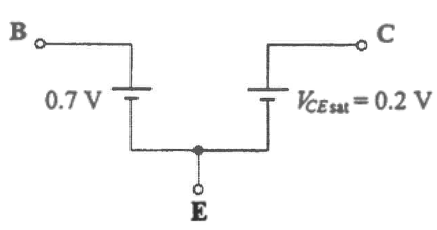
\includegraphics[width=1\linewidth]{img/3/BJT/saturation.png}
            \label{img:saturation-BJT}
        \end{center}
    \end{minipage}
    }
\end{center}

\footnotetext[5]{%
    ``Saturation means something completely different in a BJT and in a MOSFET. The saturation mode of operation of the BJT is analogous to the triode region of operation of the MOSFET. On the other hand, the saturation region of operation of the MOSFET corresponds to the active mode of BJT operation.''\cite{sedra-smith:microelectronic-circuits}
}

%//==============================--@--==============================//%
\vspace{-2.5em}
\paragraph[3.1.1.3 Modo de Corte (\textit{Cutoff})]{$\pmb{\star}$ Modo de Corte (\textit{Cutoff})}\mbox{}

\vspace{-1.25em}
\begin{center}
    \begin{minipage}{0.65\linewidth}
        $i_C = i_B = i_E = 0$ e o circuito equivalente é aberto.
        
        $v_{BE} < 0$ (tipicamente consideramos $v_{BE} < 0.5$V mediante a curva característica), e $v_{CE} > 0$. Como já explicitado $v_{BC} < 0$ já que possui polarização inversa.

        O circuito comporta-se como um \underline{interruptor aberto}.
    \end{minipage}%
    \qquad
    \begin{minipage}{0.25\linewidth}
        \begin{center}
            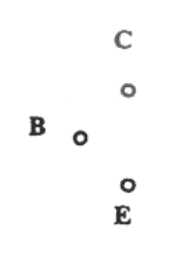
\includegraphics[width=0.6\textwidth]{img/3/BJT/cutoff.png}
            \label{img:cutoff-BJT}
        \end{center}
    \end{minipage}
\end{center}


%//==============================--@--==============================//%
\vspace{-2.0em}
\paragraph[3.1.1.4 TL;DR: Análise]{$\pmb{\star}$ TL;DR: Análise}\mbox{}\\[4pt]
Normalmente, é imediato verificar se o transístor se encontra em \underline{corte} ($v_\textit{BE} < 0.5$V) ou em \underline{condução} ($v_\textit{BE} \simeq 0.7$V). Torna-se mais difícil determinar se o circuito impõe o transístor, em condução, na ZAD ou na Zona de Saturação. Na prática \underline{assume-se uma das hipóteses} e verifica-se se os valores das tensões e correntes resultantes desta análise são congruentes com a suposição feita; caso não sejam, é porque se trata da outra zona de funcionamento (havendo que repetir a análise para obter os valores apropriados das tensões e correntes).

\begin{mdframed}
    \begin{itemize}[leftmargin=*]
        \item[] \textbf{(i) Corte:} \\
        $v_\textit{BE} \le 0.5$V; $i_B = 0$ e $i_C = 0 \implies i_E = 0$
        
        \item[] \textbf{(ii) Saturação:} \\
        $v_\textit{BE} \simeq 0.7$V; $v_\textit{CE} \le v_\textit{BE} \implies i_C < \beta i_B$
        $$
        \boxed{%
            v_\textit{CE} =
            \left\{\begin{aligned}
                v_\textit{BE} \simeq 0.7\text{V} &\rightarrow \text{limiar de saturação}\\
                V_\textit{CEsat} = 0.2\text{V} &\rightarrow \text{transístor profundamente saturado}
            \end{aligned}\right.
        }
        $$
        
        \item[] \textbf{(iii) Ativo (ZAD):} \\
        $v_\textit{BE} \simeq 0.7$V; $v_\textit{CE} > v_\textit{BE} \implies i_C = \beta i_B \;\land\; i_C = \alpha\, i_E$
        $$
        \boxed{%
            i_C = I_S(e^{\frac{v_\textit{BE}}{V_T}} - 1) \simeq I_S\, e^{\frac{v_\textit{BE}}{V_T}} \;\text{com } V_T = \frac{kT}{q} \simeq 25\,\text{mV ($@290$K)} 
        }
        $$
    \end{itemize}
\end{mdframed}

\noindent \underline{\textbf{Nota:}} O transístor é um elemento não-linear; cada zona de funcionamento pode ser aproximada por um esquema equivalente linear. A partir do momento em que se sabe a zona de funcionamento, basta aplicar as técnicas de análise de circuitos lineares para obter as correntes e tensões.

%//==============================--@--==============================//%
\newpage
\subsubsection[3.1.2 Curvas características i-v]{$\pmb{\rightarrow}$ Curvas características $\mathbf{i-v}$}
%//==============================--@--==============================//%
\vspace{-0.5em}
\paragraph[3.1.2.1 Característica iC-vBE e efeito da temperatura]{$\pmb{\star}$ Característica $\mathbf{i_C-v_{BE}}$ e efeito da temperatura}\mbox{}

\vspace{-0.5em}
\begin{figure}[H]
    \begin{subfigure}[b]{0.475\linewidth}
        \centering
        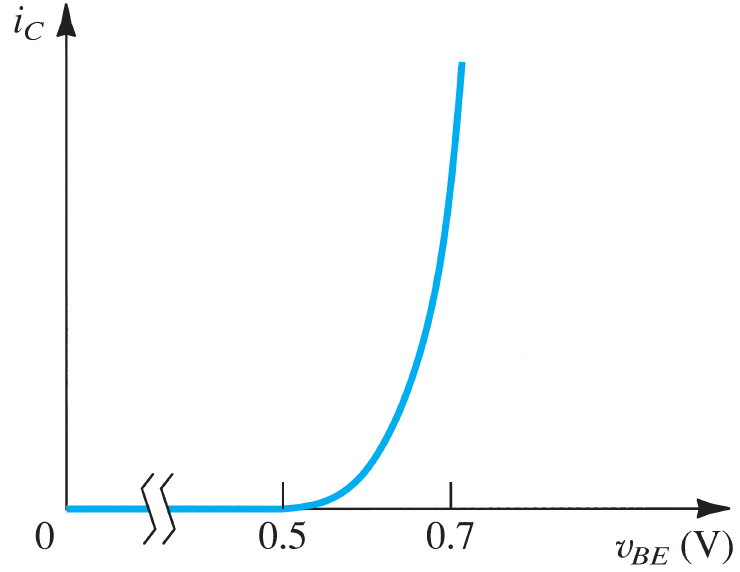
\includegraphics[width = 0.9\linewidth]{img/3/BJT/iC-vBE.png}
        \caption{Característica $i_C-v_\textit{BE}$ (npn). ``For $v_\textit{BE}$ smaller than about $0.5$V, the current is negligibly small (...)''\cite{sedra-smith:microelectronic-circuits}}
        \label{fig:i-vBE}
    \end{subfigure}\hfill
    \begin{subfigure}[b]{0.475\linewidth}
        \centering
        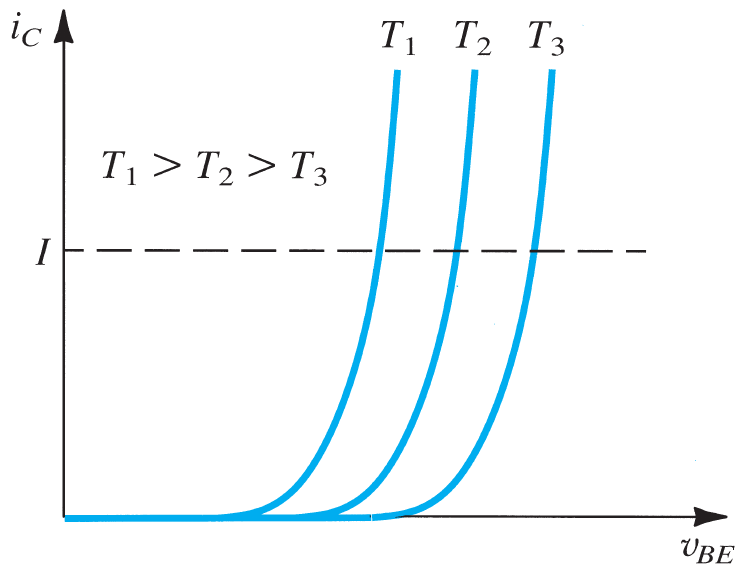
\includegraphics[width = 0.9\linewidth]{img/3/BJT/iC-vBE-T.png}
        \caption{``\textbf{Effect of temperature} (...) At a constant emitter current (broken
line), $v_\textit{BE}$ changes by $-2 \text{mV/\textdegree{C}}$.''\cite{sedra-smith:microelectronic-circuits}}
        \label{fig:i-vBE-T}
    \end{subfigure}%%
    \caption{Característica $i_C-v_\textit{BE}$}
    \label{fig:iC-vBE}
\end{figure}

\vspace{-1.75em}
\begin{quote}\small
    ``(...) over most of the normal current range $v_\textit{BE}$ lies in the range of $0.6$V to $0.8$V. In performing first-order DC calculations, we normally will assume that $V_\textit{BE} = 0.7$V, which is similar to the approach used in the analysis of diode circuits.''\cite{sedra-smith:microelectronic-circuits}
\end{quote}

%//==============================--@--==============================//%
\vspace{-1.5em}
\paragraph[3.1.2.2 Efeito de Early]{$\pmb{\star}$ Efeito de Early}\mbox{}

\vspace{-1em}
\begin{figure}[H]
    \centering
    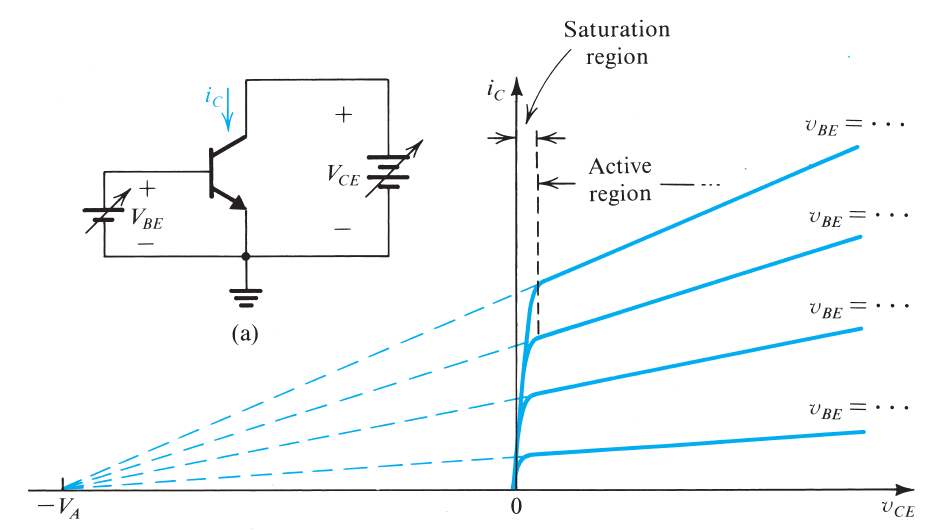
\includegraphics[width = 0.75\linewidth]{img/3/BJT/Early.png}
    \caption{Característica $i_C-v_{CE}$}
    \label{fig:Early}
\end{figure}

\vspace{-1.75em}
\begin{quote}\small
    ``At a given value of $v_{BE}$, increasing $v_{CE}$ increases the reverse-bias voltage on the collector–base junction, and thus increases the width of the depletion region of this junction. This in turn results in a decrease in the effective base width $W$. Recalling that $I_S$ is inversely proportional to $W$,\textbf{ we see that $I_S$ will increase and that $i_S$ increases proportionally}. This is the Early effect. For obvious reasons, it is also known as the base-width modulation effect.''\cite{sedra-smith:microelectronic-circuits}
\end{quote}

\noindent As curvas características atravessam o eixo das abcissas num ponto comum, $v_{CE} = -V_A$, onde $V_A$ é denominada de tensão de Early\footnotemark[6]. Esta dependência linear pode ser incutida na equação característica $i_C - v_{BE}$ da seguinte forma:
$$
    I_S\, \propto\, \frac{1}{W} \implies \boxed{i_C = I_S\, e^{v_{BE}/V_T} \left(1 + \frac{v_{CE}}{V_A}\right)}
$$

\footnotetext[6]{%
    ``The voltage $V_A$, a positive number, is a parameter for the particular BJT. As noted earlier, it is called the \textbf{Early voltage}, after J. M. Early, the engineering scientist who first studied this phenomenon''\cite{sedra-smith:microelectronic-circuits}
}

%//==============================--@--==============================//%
\newpage
\subsubsection[3.1.3 Esquema incremental]{$\pmb{\rightarrow}$ Esquema incremental}

Os circuitos analógicos destinam-se, na maior parte dos casos, a realizar operações \underline{lineares}. Nestes circuitos, \underline{pretende-se que os transístores se encontrem na ZAD}, podendo as suas tensões e correntes variar, mas sempre de modo a que o modo de funcionamento permaneça sobre um troço linear das curvas que caracterizam o funcionamento do transístor na ZAD.

Os sinais de interesse são as \underline{pequenas variações} das tensões e correntes, e não o total.

\begin{mdframed}
    \noindent Diz-se que o circuito está em \underline{repouso quando as componentes variáveis são nulas}. As componentes contínuas definem o \textbf{ponto de funcionamento em repouso} (PFR).
\end{mdframed}

\vspace{-0.25em}
\begin{figure}[H]
    \centering
    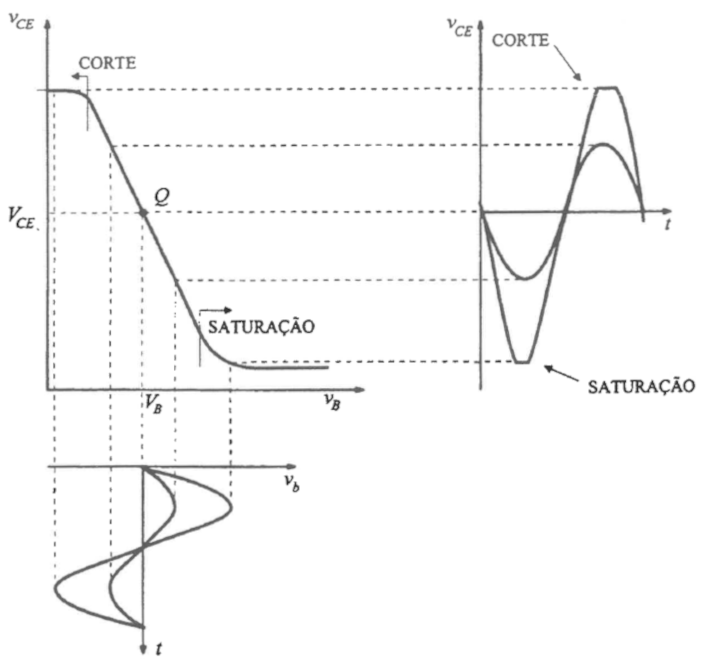
\includegraphics[width = 0.6\linewidth]{img/3/BJT/funcionamento-dinamico.png}
    \caption{Funcionamento dinâmico linear e não-linear \cite{medeiros:CTBM}}
    \label{fig:funcionamento-dinamico}
\end{figure}

\noindent Quando a tensão de saída não tem a forma da tensão de entrada, então há \underline{distorção}, resultante do funcionamento não-linear. A \underline{margem dinâmica} é dada pelas amplitude máximas incrementais para o qual ainda não ocorre distorção. Este valor é normalmente maximizado para o PFR localizado a meio do troço linear da característica (neste caso o corte e a saturação manifestam-se para as mesmas amplitudes da tensão de entrada).
\vspace{1em}\hrule\vspace{1em}
\noindent O uso de um \underline{esquema equivalente incremental} (interessa-nos o \textbf{esquema em $\pmb{\pi}$ híbrido}) pressupõe uma análise do funcionamento dinâmico linear do circuito, que ocorre quando as componentes variáveis têm amplitude limitada, de modo a que o ponto de funcionamento do transístor permaneça sobre um troço aproximadamente linear das suas características. Diz-se, neste caso, que o circuito tem \textbf{sinais fracos}.

\vspace{1 em}
\noindent Neste funcionamento o transístor é caracterizado por \textbf{parâmetros incrementais}, que caracterizam o seu modelo equivalente, $g_m$ e $r_\pi$:
$$
    \boxed{i_c = g_m\, v_{\pi}} \quad\land\quad \boxed{v_{\pi} = r_\pi\, i_b}
$$

\newpage
\begin{mdframed}
    \noindent Supondo que $i_C = I_C + i_c$ e $v_{BE} = V_{BE} + v_{be}$, e relembrando a característica $i_C-v_{BE}$ já discutida anteriormente, obtemos (desprezando o efeito de Early):

    \vspace{-0.25em}
    \begin{center}
        \begin{minipage}{0.3\linewidth}
            $$
                \boxed{i_C = I_se^{(V_{BE} + v_{be})/ V_T}}  \;\rightarrow\;
            $$
        \end{minipage}%
        \raisebox{-0.75em}{%
        \begin{minipage}{0.6\linewidth}
            A exponencial associada a $v_{be}$ é aproximada por $1 + v_{eb}/V_T$, já que $v_{be}$ se trata de um sinal fraco ($v_{eb} \ll V_T\:$ e $\:[e^x \simeq 1-x\;\text{\small (Maclaurin de 1\textordfeminine{}. ordem)}]$).
        \end{minipage}}
    \end{center}

    \vspace{-0.5em}
    \noindent Finalmente, admitimos que:
    $$
        i_C = I_C + i_c = I_se^{V_{BE}/ V_T}(1 + v_{eb}/V_T)\;
        \rightarrow\; \boxed{i_c = \dfrac{I_C}{V_T} v_{eb}}
    $$
\end{mdframed}

\renewcommand*{\thefootnote}{\fnsymbol{footnote}}
\footnotetext[4]{%
    \textbf{Nota:} As correntes e tensões no transístor têm uma componente contínua e uma componente variável. De acordo com a notação utilizada na literatura, o \textbf{valor total} será representado por uma letra minúscula com índice maiúsculo (e.g.: $v_B$), o \textbf{valor em repouso} ou \textbf{componente contínua} será representado por uma letra maiúscula com índice maiúsculo (e.g.: $V_B$) e o \textbf{valor incremental} por uma letra minúscula com índice minúsculo (e.g.: $v_b$).
}
\renewcommand*{\thefootnote}{\arabic{footnote}}

\noindent Donde resulta que a \textbf{transcondutância} é:
$$
    \boxed{g_m = \left.\frac{\partial i_C}{\partial v_\textit{BE}}\right|_{v_\textit{BE} = V_\textit{BE};\, v_\textit{CE} = V_\textit{CE}} \simeq I_C/V_T}
$$

\noindent O parâmetro $g_m$ depende apenas do \textbf{ponto de funcionamento em repouso} (PFR). Na caracterização da maior parte dos circuitos lineares, $g_m$, tem um papel determinante (e.g., o ganho de tensão do andar de emissor comum é proporcional a $g_m$). Interessa, por isso, que o valor em repouso seja bem definido e estável.

\begin{mdframed}
    \noindent Para determinar $r_\pi$ consideramos o transístor na zona ativa:
    $$
        i_c = \beta i_b
    $$
    \noindent Recordando a relação linear entre $i_c$ e $g_m$:
    $$
        v_{\pi} = r_\pi i_b = \frac{\beta}{g_m} i_b \implies \boxed{r_\pi = \frac{\beta}{g_m}}
    $$
    \noindent Note-se que $r_\pi$, depende do ponto de funcionamento em repouso (tal como $g_m$) e também da tecnologia (através de $\beta$).
\end{mdframed}

\noindent Na realidade, $i_C$ também depende de $v_\textit{CE}$, embora de modo não muito acentuado, como mencionado anteriormente. Isto constitui o \textbf{efeito de Early}. As características $i_C(v_\textit{CE})$ com $v_{BE}$ constante são aproximadamente retilíneas na zona ativa, mas não são horizontais; se fossem prolongadas para valores negativos de $v_\textit{CE}$ cortariam o eixo das abcissas em $-V_A$. Assim, a equação do transístor considerando o efeito de Early é:
$$
    \boxed{i_C = I_S\, e^{v_{BE}/V_T} \left(1 + \frac{v_{CE}}{V_A}\right)}
$$
O parâmetro $V_A$ (tensão de Early) está normalmente compreendido entre $50$ e $150$V. Quando se despreza o efeito de Early $V_A \to +\infty$.

{\setlength{\fboxrule}{2pt} 
\begin{minipage}{\linewidth}
    \raisebox{1.75em}{%
    \begin{minipage}[t]{0.475\linewidth}
        \begin{figure}[H]
            \centering
            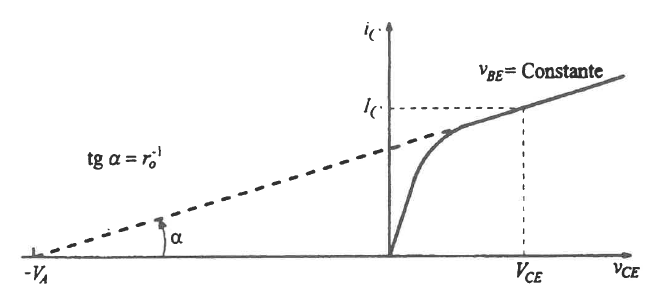
\includegraphics[width=\linewidth]{img/3/BJT/efeito-Early.png}
            \captionsetup{skip=-2pt}
            \caption{Efeito de Early \cite{medeiros:CTBM}}
            \label{fig:efeito-early-declive}
        \end{figure}
    \end{minipage}}\hspace*{1pt}
    \noindent\fbox{%
    \begin{minipage}[t]{0.46\linewidth} \small
        A inclinação da característica é:
        $$
            r_o^{-1} = \left.\frac{\partial i_C}{\partial v_\textit{CE}}\right|_{v_\textit{BE} = V_\textit{BE};\, v_\textit{CE} = V_\textit{CE}} = \frac{I_C}{V_A + V_\textit{CE}}
        $$
        e como $V_A \gg V_\textit{CE}$ tem-se, aproximadamente:
        $$
            r_o \simeq \frac{V_A}{I_C}\; \text{\small (novo parâmetro incremental)}
        $$
    \end{minipage}}
\end{minipage}
}

\vspace{0.25em}
\noindent A expressão da transcondutância \underline{não é alterada quando se considera o efeito de Early}. Quando se considera este efeito, há que introduzir no esquema incremental do transístor a resistência $r_o$ entre o coletor e o emissor de modo a traduzir a influência de $v_\textit{ce}$ sobre $i_c$.

Usualmente o efeito de Early afeta pouco o funcionamento em repouso, mas pode afetar muito o funcionamento dinâmico (principalmente no caso dos circuitos integrados).

\begin{figure}[H]
    \begin{subfigure}[b]{0.5\linewidth}
        \centering
        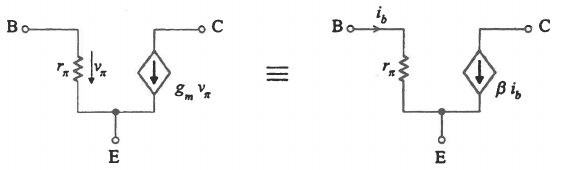
\includegraphics[width = \linewidth]{img/3/BJT/esquema-incremental.png}
        \caption{Esquema incremental em $\pi$ \cite{medeiros:CTBM}}
        \label{fig:esquema-incremental}
    \end{subfigure}%%
    \begin{subfigure}[b]{0.5\linewidth}
        \centering
        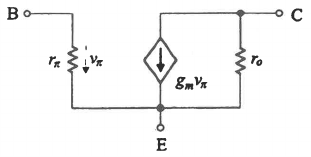
\includegraphics[width = 0.55\linewidth]{img/3/BJT/esquema-incremental-Early.png}
        \caption{Esquema incremental considerando o efeito de Early \cite{medeiros:CTBM}}
        \label{fig:esquema-incremental-Early}
    \end{subfigure}
    \caption{Esquemas incrementais em $\pi$}
    \label{fig:esquemas-incrementais}
\end{figure}

\vspace{-0.5em}
\noindent Dado que $r_o \simeq V_A/I_C$ e $g_m = I_C/V_T$,  vem que: 
$$
    \frac{r_o}{g_m^{-1}} = \frac{V_A}{V_T}
$$
\noindent Como $r_\pi = \beta\, g_m^{-1}$, para os valores usuais dos parâmetros incrementais, podemos concluir:
$$
    \boxed{r_o \gg r_\pi \gg g_m^{-1}}
$$

\begin{mdframed} \small
    \noindent O \textbf{esquema incremental do transístor} é muito útil para analisar circuitos em regime dinâmico linear (com \textbf{sinais fracos}). Esta análise efectua-se, com comodidade, substituindo o circuito pelo seu esquema equivalente do ponto de vista incremental, o qual se obtém do seguinte modo:
    \begin{enumerate}[leftmargin=*] \small
        \item Os transístores são substituídos pelo seu esquema incremental. Se, para além dos transístores, existirem outros dispositivos não-lineares (por exemplo, díodos), estes são também substituídos pelos seus esquemas incrementais.
    
        \item As fontes de tensão contínua são substituídas por curto-circuitos, pois a componente incremental de uma tensão constante é nula; as fontes de corrente contínua são substituídas por circuitos abertos, com análoga justificação.
        
        \item Os elementos lineares (resistências, condensadores, etc) mantêm-se, uma vez que eles coincidem com o seu esquema incremental (as equações que os descrevem em termos dos valores totais são lineares e, por isso, são aplicáveis aos valores incrementais).
    \end{enumerate}
\end{mdframed}

\renewcommand*{\thefootnote}{\fnsymbol{footnote}}
\footnotetext[4]{%
    ``E importante notar que \textbf{os esquemas incrementais dos transístores \textit{pnp} e \textit{npn} são idênticos}. Pode considerar-se que os sentidos das correntes e tensões incrementais são os mesmos nos dois tipos de transístores (embora tal não seja verdade para os valores totais).''\cite{medeiros:CTBM}
}
\renewcommand*{\thefootnote}{\arabic{footnote}}

%//==============================--@--==============================//%
\subsubsection[3.1.4 Polarização Estabilizada]{$\pmb{\rightarrow}$ Polarização Estabilizada}



%//==============================--@--==============================//%